\chapter*{2 Versuchsdurchführung und Auswertung}
\addcontentsline{toc}{chapter}{2 Versuchsdurchführung und Auswertung}
\setcounter{chapter}{2}
\setcounter{section}{0}
\setcounter{subsection}{0}

\section{Versuch: Brennweite einer Sammellinse}

\subsection{Versuchsaufbau und -durchführung}

    \bem{
        \begin{itemize}
            \item
                Linsenformel: $\frac{1}{f} = \frac{1}{g} + \frac{1}{b}$
            \item
                Gegenstands- und Bildgröße: $\frac{B}{G} = \frac{b}{g}$
            \item
                $4f = g + b$
        \end{itemize}
    }

    \subsubsection{Teil 1}
    
        Für den ersten Teil des Versuchs wird die Lampe auf der Schiene befestigt und die Linse zwischen Lampe und Schirm bewegt, bis die Brennweite der Linse gefunden wurde. Nun wird der Abstand zwischen Linse und Schirm gemessen um die Brennweite zu bestimmen.

        Die Messung ergab eine Brennweite von $f \approx 80\ \mathrm{mm}$.

    \subsubsection{Teil 2}
    
        Für den zweiten Teil des Versuchs wird die Lampe ca. $3 - 4\ \mathrm{m}$ vom Schirm entfernt platziert. Zwischen Lampe und Schirm wird nun eine Schablone und die Linse platziert. Schablone und Linse müssen nun so verschoben werden, dass einmal eine Vergrößerung und einmal eine Verkleinerung der Schablone auf dem Schirm entsteht.

        Die Messungen ergeben:

        \begin{table}[h]
            \begin{center}
                \begin{tabular}{|l|l|l|}
                    \hline
                    Werte & Versuch 1 & Versuch 2\\
                    \hline
                    $G$ & $30\ \mathrm{mm}$ & $30\ \mathrm{mm}$ \\
                    $g$ & $475\ \mathrm{mm}$ & $95\ \mathrm{mm}$ \\
                    $B$ & $6\ \mathrm{mm}$ & $147\ \mathrm{mm}$ \\
                    $b$ & $94\ \mathrm{mm}$ & $468\ \mathrm{mm}$\\
                    \hline
                \end{tabular}
            \end{center}
        \end{table}

        Mit der Linsenformel erhält man:

        $$
        \begin{aligned}
            \frac{1}{f} &= \frac{1}{g} + \frac{1}{b}\\
            &\approx \frac{1}{475\ \mathrm{mm}} + \frac{1}{94\ \mathrm{mm}}\\
            &\approx 0,013\ \frac{1}{\mathrm{mm}}
        \end{aligned}
        $$

        Daraus folgt: $f \approx = 78,5\ \mathrm{mm}$.
        
        Analog für die zweiten Messdaten:

        $$
        \begin{aligned}
            \frac{1}{f} &= \frac{1}{g} + \frac{1}{b}\\
            &\approx \frac{1}{95\ \mathrm{mm}} + \frac{1}{468\ \mathrm{mm}}\\
            &\approx 0,013\ \frac{1}{\mathrm{mm}}
        \end{aligned}
        $$

        Daraus folgt: $f \approx 79,0\ \mathrm{mm}$.

    \subsubsection{Teil 3}
    
        Für den drittel Teil müssen die Schablone und die Linse so verschoben werden, dass es nur noch einen Punkt gibt, an dem das Bild scharf auf dem Schirm zu erkennen ist. Hier kann man nun den Abstand zwischen Schablone und Schirm messen und erhält so die Brennweite der Linse:

        $$
        \begin{aligned}
            4f &= b + g\\
            &\approx 318\ \mathrm{mm}
        \end{aligned}
        $$

        Daraus folgt nun: $f \approx 79,5\ \mathrm{mm}$.

    \subsubsection{Teil 4}
    
        Für den letzten Teil wird der Schirm durch einen Spiegel ausgestauscht, sodass die parallelen Strahlen nach der Linse reflektiert werden und auf dem Rückweg in der Linse gebündelt werden. Das Bild sollte auf der Rückseite der Schablone zu sehen sein. Misst man nun den Abstand zwischen Schablone und Linse erhält man die Brennweite der Linse.

        Die Messung ergab eine Brennweite von $f \approx 80\ \mathrm{mm}$.

    \subsection{Diskussion}

        Wir wissen das die Linse eine Brennweite von $80\ \mathrm{mm}$ hat und die Abweichungen zu den ersten drei Teilversuchen nur $1,5\ \mathrm{mm}$ und $0,5\ \mathrm{mm}$ betragen. Die Abweichung zum letzten Teilversuch beträgt sogar $0\ \mathrm{mm}$. Die Schwankungen lassen sich auf kleinere Messfehler zurückführen, die sich darauf zurückführen lassen, dass die Messungen mit einem Lineal durchgeführt wurden und dass sich die Hauptebene der Linse schlecht im Rahmen bestimmen lässt und grob abgeschätzt werden musste.

        Die Messungen zeigen, dass die Herstellerangaben mit den Messwerten übereinstimmen, dass sich die Werte nicht signifikant unterscheiden und nicht genauer bestimmt werden können.

\newpage

\section{Versuch: Linsenkombinationen}

    \subsection{Versuchsaufbau und -durchführung}

        Bei diesem Versuch wird der gleiche Versuchsaufbau wie bei Versuch 1 Teil 3 verwendet. Der einzige Unterschied ist, dass die Linse nun aus 2 Teilen besteht. Der erste Teil der Linse ist eine Zerstreuungslinse, der zweite Teil eine Sammellinse. Die beiden Linsen sind so nah aneinander platziert, dass sie als eine Linse betrachtet werden können.

        Wird nun die gleiche Messung wie bei Versuch 1, Teil 3 angewendet, so erhält man die Brennweite der Kombination aus Zerstreuungs- und Sammellinse:

        $$
        \begin{aligned}
            4f_{\mathrm{ges}} &= b + g\\
            &\approx 624\ \mathrm{mm}
        \end{aligned}
        $$

        Daraus folgt nun: $f_{\mathrm{ges}} \approx 156\ \mathrm{mm}$.

        Nimmt man nun die Brennweite der Sammellinse als gegeben an ($f_{1} = 80\ \mathrm{mm}$), so kann man mit der Formel für Linsenkombination die Brennweite der Zerstreuungslinse bestimmen:

        $$
        \begin{aligned}
            \frac{1}{f_{2}} &= \frac{1}{f_{\mathrm{ges}}} - \frac{1}{f_{1}}\\
            &\approx \frac{1}{156\ \mathrm{mm}} - \frac{1}{80\ \mathrm{mm}}\\
            &\approx -0,006\ \frac{1}{\mathrm{mm}}
        \end{aligned}
        $$

        Daraus folgt: $f_{2} \approx -164\ \mathrm{mm}$.

    \subsection{Diskussion}

        Die Ergebnisse dieses Versuchs sind um einiges ungenauer als die Ergebnisse des Versuches davor. Dies könnte daran liegen, dass mehr Abschätzungen vorgenommen wurden, wie z.B. die Abschätzung, dass wir die beiden Linsen als eine Linse betrachten. Hier befinden sich zwischen den beiden Linsen ein Raum, welcher die Messungen verfälschen könnte. Außerdem wurde die Hauptebene der Linse wieder nur grob abgeschätzt. Zudem kommen die groben Messungen mit Lineal, welche nur auf Millimeter genau gemessen werden können.

\newpage

\section{Versuch: Aufbau und Charakterisierung eines Mikroskops}

    \subsection{Versuchsaufbau und -durchführung}

        Bei diesem Versuch wird schrittweise ein Mikroskop aufgebaut. Zuerst wird eine schwachere Lichtquelle als in den letzten Versuchen gewählt, sodass die resultierenden Strahlen keine Schäden anrichten können. Als nächsten werden zwei Linsen ($f_{\mathrm{obj}} = 16\ \mathrm{mm}, f_{\mathrm{Ok}} = 40\ \mathrm{mm}$) gewählt und auf zwei Metalstäben befestigt. Der Abstand der beiden Linsen wird hier so groß wie möglich gewählt, sodass wir einen starken Vergrößerungseffekt erzielen. Ist der Aufbau korrekt, so lässt sich eine Zahlenskala vergrößert erkennen.

        \begin{center}
            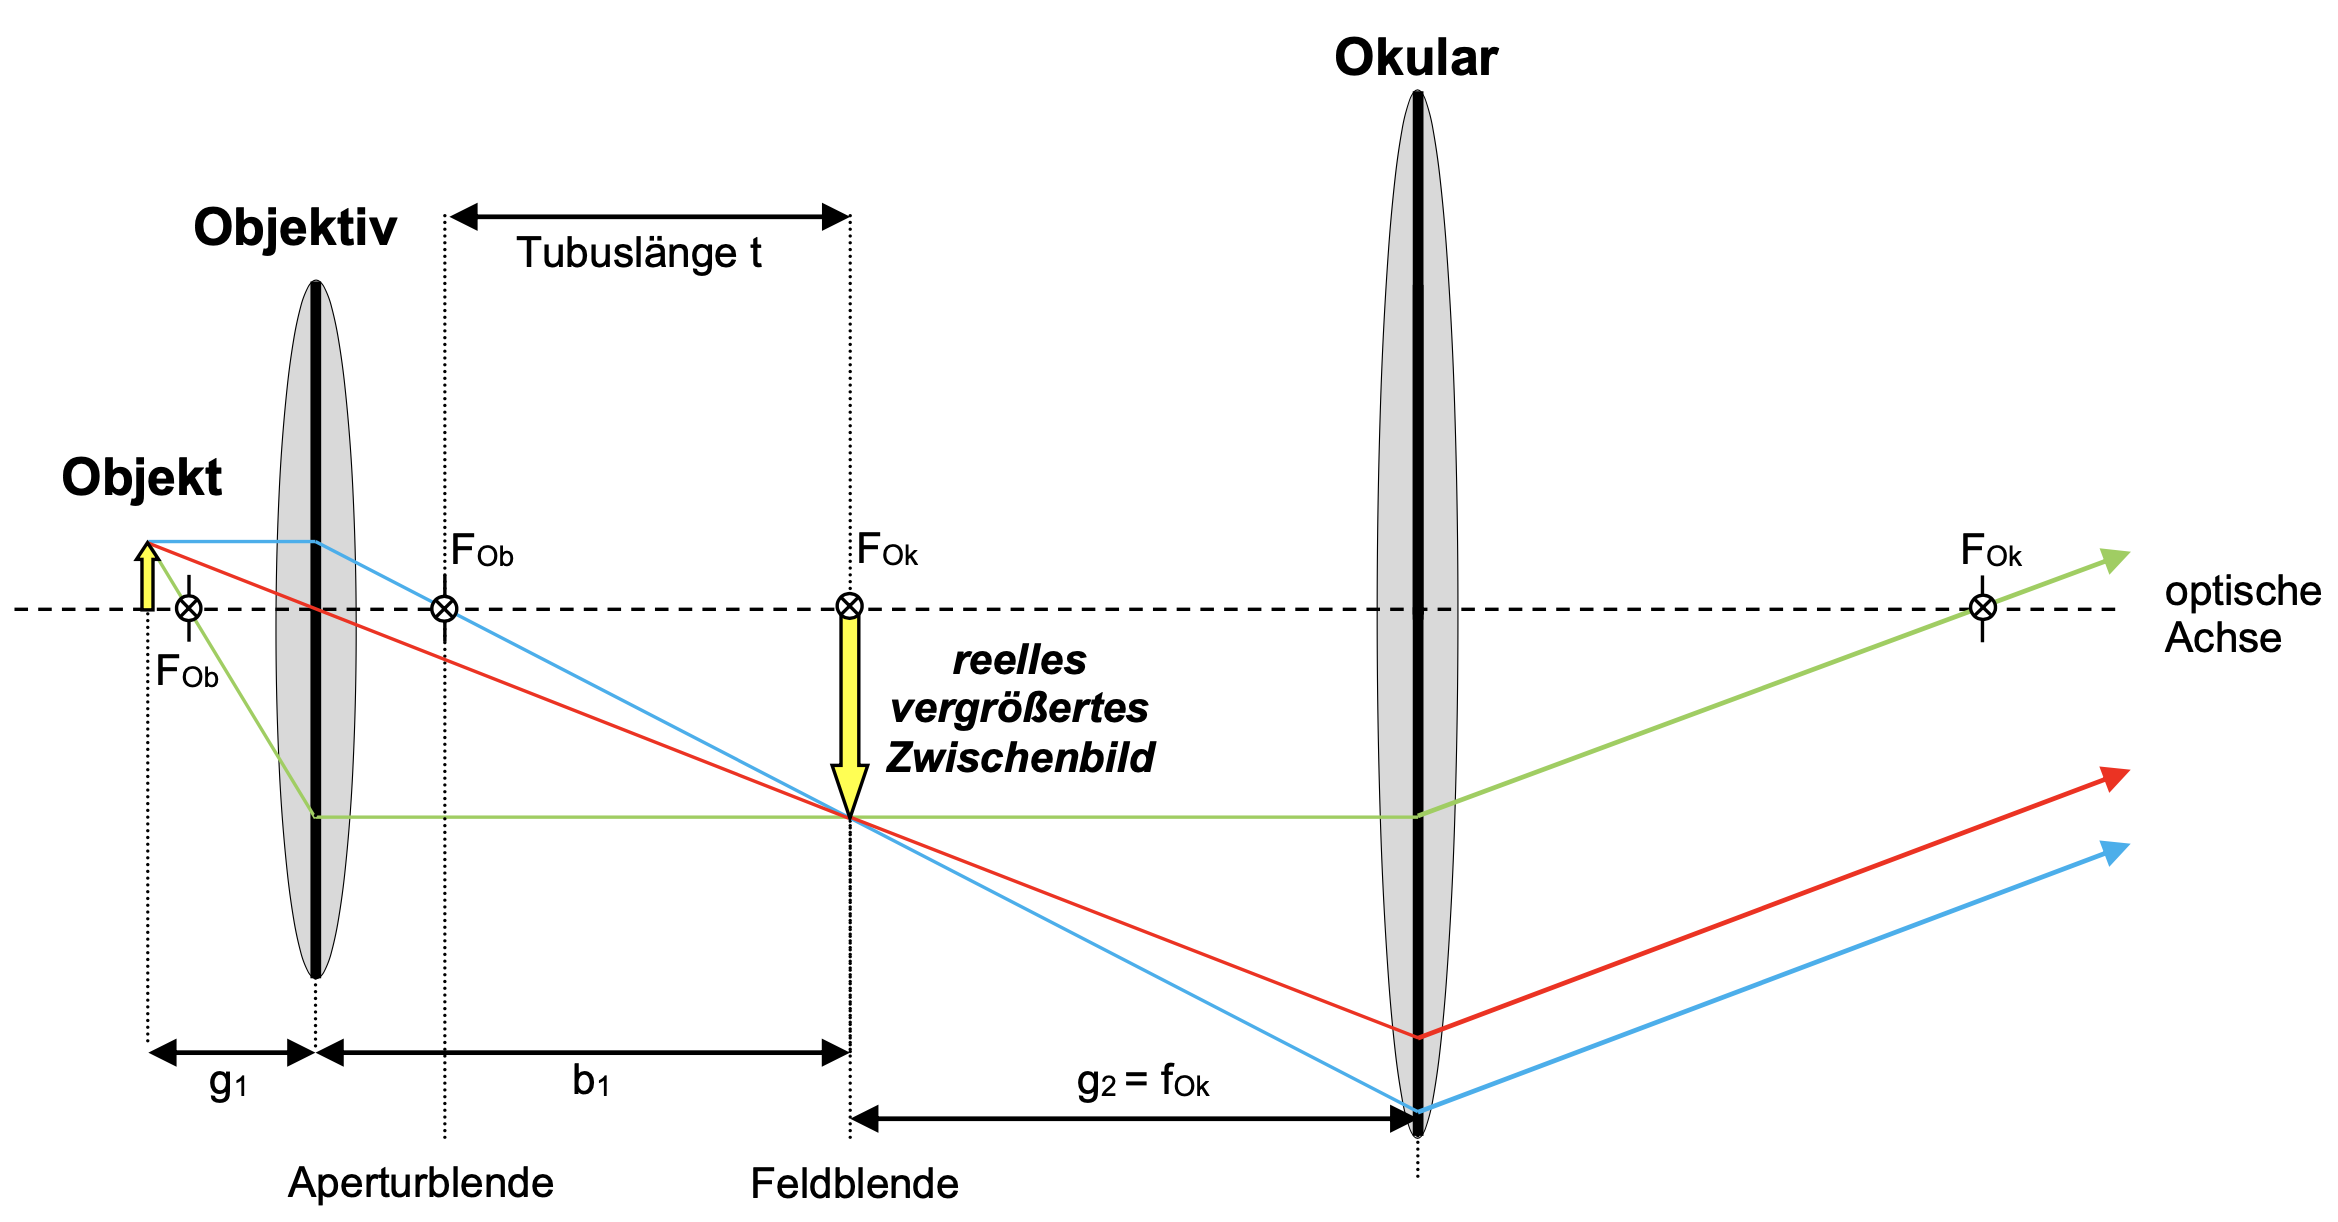
\includegraphics[width=0.9\textwidth]{skizze.png}
        \end{center}

        \subsubsection{Teil 1}
        
            Für den ersten Teil wird nun eine Blende bei $f_{\mathrm{obj}}$ und bei $f_{\mathrm{Ok}}$ eingesetzt und diese verschlossen und wieder geöffnet.

            Es lässt sich beobachten, dass durch das Schließen der (Apertur-) Blende, also an der Position $f_{\mathrm{obj}}$, sich der Bildausschnitt nicht verändert, sondern nur die Helligkeit. Je weiter sich die Blende verschließt, desto dunkler wird das Bild. Bei der (Feld-) Blende, also an der Position $f_{\mathrm{Ok}}$, verändert sich der Bildausschnitt. Je weiter sich die Blende verschließt, desto kleiner wird der Bildausschnitt, wobei sich die Helligkeit nicht verädnert.

            In der Praxis kann die Aperturblende für die Helligkeitseinstellung verwendet werden und die Feldblende für den Bildausschnitt.
        
        \subsubsection{Teil 2}

            Im zweiten Teil soll die Vergrößerung des Mikroskops bestimmt werden. Zuerst mit Hilfe der Geometrie des Mikroskops und dann mit Hilfe eines Maßstabs.

            Für die Berechnung mit Hilfe der Geometrie werden einige Messungen benötigt. Diese sind in der folgenden Tabelle aufgelistet:

            \begin{table}[h]
                \begin{center}
                    \begin{tabular}{|l|l|}
                        \hline
                        Werte & Messung\\
                        \hline
                        $f_{\mathrm{obj}}$ & $16\ \mathrm{mm}$\\
                        $f_{\mathrm{Ok}}$ & $40\ \mathrm{mm}$\\
                        $t$ & $226\ \mathrm{mm}$\\
                        $s_{0}$ & $250\ \mathrm{mm}$\\
                        \hline
                    \end{tabular}
                \end{center}
            \end{table}

            Mit diesen Werten lässt sich nun die Vergrößerung des Mikroskops berechnen:

            $$
            \begin{aligned}
                v_{m} &= \frac{t \cdot s_{0}}{f_{\mathrm{Ok}} \cdot f_{\mathrm{Obj}}}\\
                &\approx \frac{226\ \mathrm{mm} \cdot 250\ \mathrm{mm}}{16\ \mathrm{mm} \cdot 40\ \mathrm{mm}}\\
                &\approx 88,3
            \end{aligned}
            $$

            Mit Hilfe eines Maßstabs, kann die Vergrößerung ebenfalls gemessen werden. Hier schaut man mit einem Auge durch das Mikroskop und mit dem anderen daran vorbei und hält einen Gegenstand mit einem Abstand von ca. $25\ \mathrm{cm}$ neben vor das andere Auge. Nun versucht man das Objekt mit der vergrößerten Skala zu vermessen:

            \begin{table}[h]
                \begin{center}
                    \begin{tabular}{|l|l|}
                        \hline
                        Werte & Messung\\
                        \hline
                        $B$ & $10\ \mathrm{mm}$\\
                        $G$ & $100\ \mathrm{\mu m}$\\
                        \hline
                    \end{tabular}
                \end{center}
            \end{table}

            Daraus folgt: $v_{m} = \frac{B}{G} = \frac{10\ \mathrm{mm}}{100\ \mathrm{\mu m}} = 100$.
        
        \subsubsection{Teil 3}
            
            Bei diesem Teil wird die Objektivvergrößerung $v_{\mathrm{Obj}}$ gemessen. Dazu wird eine weitere Strichskala in die Zwischenbildebende eingesetzt und die Vergrößerung gemessen. Die zweite Strichskala hat ebenfalls einen Strichabstand von $50\ \mathrm{\mu m}$.

            Die \glqq Messung\grqq ergab, dass $14$ kleinere Striche der kleineren Skala zwischen zwei Striche in der größeren Skala passen. Daraus folgt, dass die Objektivvergrößerung $14$ beträgt.

            Mit Hilfe der Okularvergrößerung, die aus der Lupengeometrie berechnet wird, lässt sich die Gesamtvergrößerung des Mikroskops berechnen:

            $$\frac{s_{0}}{f_{\mathrm{Ok}}} = \frac{250\ \mathrm{mm}}{40\ \mathrm{mm}} = 6,25.$$

            Daraus lässt sich nun die Gesamtvergrößerung des Mikroskops berechnen:

            $$v_{m} \approx v_{\mathrm{Obj}} \cdot v_{\mathrm{Ok}} \approx 14 \cdot 6,25 \approx 87,5.$$

    \subsection{Diskussion}
        
        Die Messung des letzten Teils unterscheidet sich nur minimal zu Teil 2a), nämlich nur $0,8$ Größeneinheiten. Die Abweichungen zu den Ergebnissen in Teil 2b) sind extremer, da die Messungen sehr ungenau ist, da die Skala sehr klein ist und die Messung mit dem Auge sehr ungenau ist. Die Skala hat eine Schrittgröße von $50\ \mathrm{\mu m}$, weshalb keine genauere Messung mit dem Auge möglich ist.

\newpage

\section{Versuch: Bestimmung von Objektgrößen mit dem Mikroskop}

    \subsection{Versuchsaufbau und -durchführung}
        
        In diesem Versuch wird der Aufbau des letzten Versuchs verwendet. Es wird die Strichskala in der Zwischenbildebende verwendet um Objekte zu vermessen.

        Wir verwenden ein Haar und halten dies and die Stelle, an der vorher die Strichskala war, welche näher an der Objektivlinse stand. Mit der anderen Strichskala, welche sind in der Zwischenbildebene befindet, kann nun das Haar vermessen werden.

        Die Messung ergab, dass ein Haar ca. $20$ kleine Striche auf der Skala einnimmt.

        Bei der neu kalibrierten Skala ist der Abstand zwischen zwei kleinen Strichen $\frac{50\ \mathrm{\mu m}}{14} \approx 3,6\ \mathrm{\mu m}$. Damit ergibt sich eine Dicke des Haares von $20 \cdot 3,6\ \mathrm{\mu m} \approx 72\ \mathrm{\mu m}$.
    
    \subsection{Diskussion}
        
        Vergleicht man die Werte der Dicke des Haares von Wikipedia, oder anderen Quellen, mit den Werten der letzten Messung, so kann man erkennen, dass die Dicke des Haares ziemlich nach an die Angaben der Quellen herankommt ($60-80\ \mathrm{\mu m}$). Da jedes Haar unterschiedlich Dick ist, können hier keine wirklichen Messfehler vermutet oder herausgearbeitet werden, da die genaue Dicke des Haares nicht bekannt ist. Da die Dicke allerdings im Rahmen der Angaben ist, kann man davon ausgehen, dass die Messung erfolgreich war.